% Created by tikzDevice version 0.10.1 on 2018-01-24 12:32:16
% !TEX encoding = UTF-8 Unicode
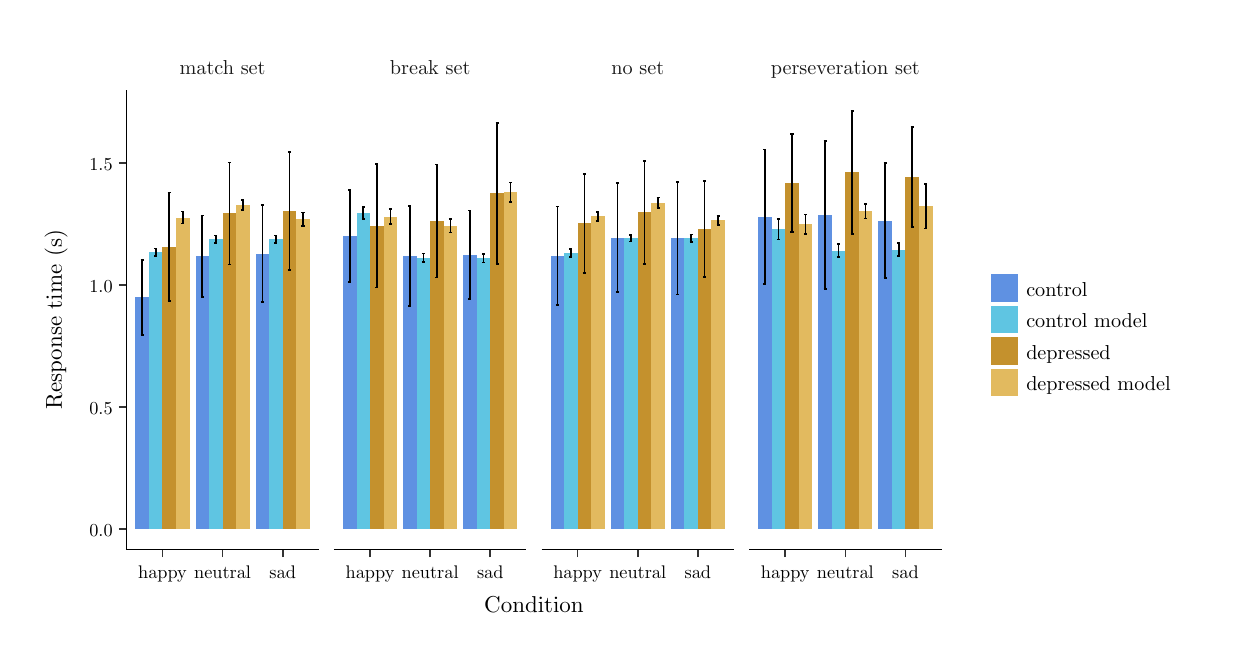
\begin{tikzpicture}[x=1pt,y=1pt]
\definecolor{fillColor}{RGB}{255,255,255}
\path[use as bounding box,fill=fillColor,fill opacity=0.00] (0,0) rectangle (433.62,216.81);
\begin{scope}
\path[clip] (  0.00,  0.00) rectangle (433.62,216.81);
\definecolor{drawColor}{RGB}{255,255,255}
\definecolor{fillColor}{RGB}{255,255,255}

\path[draw=drawColor,line width= 0.6pt,line join=round,line cap=round,fill=fillColor] (  0.00,  0.00) rectangle (433.62,216.81);
\end{scope}
\begin{scope}
\path[clip] ( 35.67, 28.22) rectangle (105.18,194.25);
\definecolor{fillColor}{RGB}{255,255,255}

\path[fill=fillColor] ( 35.67, 28.22) rectangle (105.18,194.25);
\definecolor{fillColor}{RGB}{226,186,95}

\path[fill=fillColor] ( 53.60, 35.77) rectangle ( 58.48,148.17);
\definecolor{fillColor}{RGB}{196,145,45}

\path[fill=fillColor] ( 48.71, 35.77) rectangle ( 53.60,137.68);
\definecolor{fillColor}{RGB}{95,197,226}

\path[fill=fillColor] ( 43.82, 35.77) rectangle ( 48.71,135.58);
\definecolor{fillColor}{RGB}{95,145,226}

\path[fill=fillColor] ( 38.93, 35.77) rectangle ( 43.82,119.35);
\definecolor{fillColor}{RGB}{226,186,95}

\path[fill=fillColor] ( 75.32, 35.77) rectangle ( 80.20,152.78);
\definecolor{fillColor}{RGB}{196,145,45}

\path[fill=fillColor] ( 70.43, 35.77) rectangle ( 75.32,149.67);
\definecolor{fillColor}{RGB}{95,197,226}

\path[fill=fillColor] ( 65.54, 35.77) rectangle ( 70.43,140.34);
\definecolor{fillColor}{RGB}{95,145,226}

\path[fill=fillColor] ( 60.65, 35.77) rectangle ( 65.54,134.25);
\definecolor{fillColor}{RGB}{226,186,95}

\path[fill=fillColor] ( 97.04, 35.77) rectangle (101.93,147.62);
\definecolor{fillColor}{RGB}{196,145,45}

\path[fill=fillColor] ( 92.15, 35.77) rectangle ( 97.04,150.56);
\definecolor{fillColor}{RGB}{95,197,226}

\path[fill=fillColor] ( 87.26, 35.77) rectangle ( 92.15,140.39);
\definecolor{fillColor}{RGB}{95,145,226}

\path[fill=fillColor] ( 82.38, 35.77) rectangle ( 87.26,135.13);
\definecolor{drawColor}{RGB}{0,0,0}

\path[draw=drawColor,line width= 0.6pt,line join=round] ( 55.50,150.34) --
	( 56.58,150.34);

\path[draw=drawColor,line width= 0.6pt,line join=round] ( 56.04,150.34) --
	( 56.04,145.99);

\path[draw=drawColor,line width= 0.6pt,line join=round] ( 55.50,145.99) --
	( 56.58,145.99);

\path[draw=drawColor,line width= 0.6pt,line join=round] ( 50.61,157.26) --
	( 51.69,157.26);

\path[draw=drawColor,line width= 0.6pt,line join=round] ( 51.15,157.26) --
	( 51.15,118.11);

\path[draw=drawColor,line width= 0.6pt,line join=round] ( 50.61,118.11) --
	( 51.69,118.11);

\path[draw=drawColor,line width= 0.6pt,line join=round] ( 45.72,136.97) --
	( 46.81,136.97);

\path[draw=drawColor,line width= 0.6pt,line join=round] ( 46.26,136.97) --
	( 46.26,134.19);

\path[draw=drawColor,line width= 0.6pt,line join=round] ( 45.72,134.19) --
	( 46.81,134.19);

\path[draw=drawColor,line width= 0.6pt,line join=round] ( 40.83,132.92) --
	( 41.92,132.92);

\path[draw=drawColor,line width= 0.6pt,line join=round] ( 41.38,132.92) --
	( 41.38,105.77);

\path[draw=drawColor,line width= 0.6pt,line join=round] ( 40.83,105.77) --
	( 41.92,105.77);

\path[draw=drawColor,line width= 0.6pt,line join=round] ( 77.22,154.54) --
	( 78.30,154.54);

\path[draw=drawColor,line width= 0.6pt,line join=round] ( 77.76,154.54) --
	( 77.76,151.02);

\path[draw=drawColor,line width= 0.6pt,line join=round] ( 77.22,151.02) --
	( 78.30,151.02);

\path[draw=drawColor,line width= 0.6pt,line join=round] ( 72.33,168.10) --
	( 73.42,168.10);

\path[draw=drawColor,line width= 0.6pt,line join=round] ( 72.87,168.10) --
	( 72.87,131.25);

\path[draw=drawColor,line width= 0.6pt,line join=round] ( 72.33,131.25) --
	( 73.42,131.25);

\path[draw=drawColor,line width= 0.6pt,line join=round] ( 67.44,141.69) --
	( 68.53,141.69);

\path[draw=drawColor,line width= 0.6pt,line join=round] ( 67.99,141.69) --
	( 67.99,138.99);

\path[draw=drawColor,line width= 0.6pt,line join=round] ( 67.44,138.99) --
	( 68.53,138.99);

\path[draw=drawColor,line width= 0.6pt,line join=round] ( 62.56,148.97) --
	( 63.64,148.97);

\path[draw=drawColor,line width= 0.6pt,line join=round] ( 63.10,148.97) --
	( 63.10,119.52);

\path[draw=drawColor,line width= 0.6pt,line join=round] ( 62.56,119.52) --
	( 63.64,119.52);

\path[draw=drawColor,line width= 0.6pt,line join=round] ( 98.94,150.02) --
	(100.03,150.02);

\path[draw=drawColor,line width= 0.6pt,line join=round] ( 99.48,150.02) --
	( 99.48,145.22);

\path[draw=drawColor,line width= 0.6pt,line join=round] ( 98.94,145.22) --
	(100.03,145.22);

\path[draw=drawColor,line width= 0.6pt,line join=round] ( 94.05,171.80) --
	( 95.14,171.80);

\path[draw=drawColor,line width= 0.6pt,line join=round] ( 94.60,171.80) --
	( 94.60,129.31);

\path[draw=drawColor,line width= 0.6pt,line join=round] ( 94.05,129.31) --
	( 95.14,129.31);

\path[draw=drawColor,line width= 0.6pt,line join=round] ( 89.16,141.72) --
	( 90.25,141.72);

\path[draw=drawColor,line width= 0.6pt,line join=round] ( 89.71,141.72) --
	( 89.71,139.05);

\path[draw=drawColor,line width= 0.6pt,line join=round] ( 89.16,139.05) --
	( 90.25,139.05);

\path[draw=drawColor,line width= 0.6pt,line join=round] ( 84.28,152.67) --
	( 85.36,152.67);

\path[draw=drawColor,line width= 0.6pt,line join=round] ( 84.82,152.67) --
	( 84.82,117.58);

\path[draw=drawColor,line width= 0.6pt,line join=round] ( 84.28,117.58) --
	( 85.36,117.58);
\end{scope}
\begin{scope}
\path[clip] (110.68, 28.22) rectangle (180.20,194.25);
\definecolor{fillColor}{RGB}{255,255,255}

\path[fill=fillColor] (110.68, 28.22) rectangle (180.20,194.25);
\definecolor{fillColor}{RGB}{226,186,95}

\path[fill=fillColor] (128.61, 35.77) rectangle (133.49,148.56);
\definecolor{fillColor}{RGB}{196,145,45}

\path[fill=fillColor] (123.72, 35.77) rectangle (128.61,145.18);
\definecolor{fillColor}{RGB}{95,197,226}

\path[fill=fillColor] (118.83, 35.77) rectangle (123.72,149.77);
\definecolor{fillColor}{RGB}{95,145,226}

\path[fill=fillColor] (113.94, 35.77) rectangle (118.83,141.48);
\definecolor{fillColor}{RGB}{226,186,95}

\path[fill=fillColor] (150.33, 35.77) rectangle (155.22,145.29);
\definecolor{fillColor}{RGB}{196,145,45}

\path[fill=fillColor] (145.44, 35.77) rectangle (150.33,146.94);
\definecolor{fillColor}{RGB}{95,197,226}

\path[fill=fillColor] (140.55, 35.77) rectangle (145.44,133.64);
\definecolor{fillColor}{RGB}{95,145,226}

\path[fill=fillColor] (135.67, 35.77) rectangle (140.55,134.33);
\definecolor{fillColor}{RGB}{226,186,95}

\path[fill=fillColor] (172.05, 35.77) rectangle (176.94,157.38);
\definecolor{fillColor}{RGB}{196,145,45}

\path[fill=fillColor] (167.16, 35.77) rectangle (172.05,156.90);
\definecolor{fillColor}{RGB}{95,197,226}

\path[fill=fillColor] (162.27, 35.77) rectangle (167.16,133.55);
\definecolor{fillColor}{RGB}{95,145,226}

\path[fill=fillColor] (157.39, 35.77) rectangle (162.27,134.78);
\definecolor{drawColor}{RGB}{0,0,0}

\path[draw=drawColor,line width= 0.6pt,line join=round] (130.51,151.22) --
	(131.59,151.22);

\path[draw=drawColor,line width= 0.6pt,line join=round] (131.05,151.22) --
	(131.05,145.90);

\path[draw=drawColor,line width= 0.6pt,line join=round] (130.51,145.90) --
	(131.59,145.90);

\path[draw=drawColor,line width= 0.6pt,line join=round] (125.62,167.48) --
	(126.70,167.48);

\path[draw=drawColor,line width= 0.6pt,line join=round] (126.16,167.48) --
	(126.16,122.87);

\path[draw=drawColor,line width= 0.6pt,line join=round] (125.62,122.87) --
	(126.70,122.87);

\path[draw=drawColor,line width= 0.6pt,line join=round] (120.73,151.94) --
	(121.82,151.94);

\path[draw=drawColor,line width= 0.6pt,line join=round] (121.27,151.94) --
	(121.27,147.60);

\path[draw=drawColor,line width= 0.6pt,line join=round] (120.73,147.60) --
	(121.82,147.60);

\path[draw=drawColor,line width= 0.6pt,line join=round] (115.84,158.14) --
	(116.93,158.14);

\path[draw=drawColor,line width= 0.6pt,line join=round] (116.39,158.14) --
	(116.39,124.81);

\path[draw=drawColor,line width= 0.6pt,line join=round] (115.84,124.81) --
	(116.93,124.81);

\path[draw=drawColor,line width= 0.6pt,line join=round] (152.23,147.74) --
	(153.31,147.74);

\path[draw=drawColor,line width= 0.6pt,line join=round] (152.77,147.74) --
	(152.77,142.85);

\path[draw=drawColor,line width= 0.6pt,line join=round] (152.23,142.85) --
	(153.31,142.85);

\path[draw=drawColor,line width= 0.6pt,line join=round] (147.34,167.40) --
	(148.43,167.40);

\path[draw=drawColor,line width= 0.6pt,line join=round] (147.88,167.40) --
	(147.88,126.49);

\path[draw=drawColor,line width= 0.6pt,line join=round] (147.34,126.49) --
	(148.43,126.49);

\path[draw=drawColor,line width= 0.6pt,line join=round] (142.45,135.22) --
	(143.54,135.22);

\path[draw=drawColor,line width= 0.6pt,line join=round] (143.00,135.22) --
	(143.00,132.05);

\path[draw=drawColor,line width= 0.6pt,line join=round] (142.45,132.05) --
	(143.54,132.05);

\path[draw=drawColor,line width= 0.6pt,line join=round] (137.57,152.41) --
	(138.65,152.41);

\path[draw=drawColor,line width= 0.6pt,line join=round] (138.11,152.41) --
	(138.11,116.26);

\path[draw=drawColor,line width= 0.6pt,line join=round] (137.57,116.26) --
	(138.65,116.26);

\path[draw=drawColor,line width= 0.6pt,line join=round] (173.95,160.91) --
	(175.04,160.91);

\path[draw=drawColor,line width= 0.6pt,line join=round] (174.49,160.91) --
	(174.49,153.85);

\path[draw=drawColor,line width= 0.6pt,line join=round] (173.95,153.85) --
	(175.04,153.85);

\path[draw=drawColor,line width= 0.6pt,line join=round] (169.06,182.29) --
	(170.15,182.29);

\path[draw=drawColor,line width= 0.6pt,line join=round] (169.61,182.29) --
	(169.61,131.51);

\path[draw=drawColor,line width= 0.6pt,line join=round] (169.06,131.51) --
	(170.15,131.51);

\path[draw=drawColor,line width= 0.6pt,line join=round] (164.18,135.11) --
	(165.26,135.11);

\path[draw=drawColor,line width= 0.6pt,line join=round] (164.72,135.11) --
	(164.72,132.00);

\path[draw=drawColor,line width= 0.6pt,line join=round] (164.18,132.00) --
	(165.26,132.00);

\path[draw=drawColor,line width= 0.6pt,line join=round] (159.29,150.73) --
	(160.37,150.73);

\path[draw=drawColor,line width= 0.6pt,line join=round] (159.83,150.73) --
	(159.83,118.82);

\path[draw=drawColor,line width= 0.6pt,line join=round] (159.29,118.82) --
	(160.37,118.82);
\end{scope}
\begin{scope}
\path[clip] (185.70, 28.22) rectangle (255.21,194.25);
\definecolor{fillColor}{RGB}{255,255,255}

\path[fill=fillColor] (185.70, 28.22) rectangle (255.21,194.25);
\definecolor{fillColor}{RGB}{226,186,95}

\path[fill=fillColor] (203.62, 35.77) rectangle (208.50,148.61);
\definecolor{fillColor}{RGB}{196,145,45}

\path[fill=fillColor] (198.73, 35.77) rectangle (203.62,146.06);
\definecolor{fillColor}{RGB}{95,197,226}

\path[fill=fillColor] (193.84, 35.77) rectangle (198.73,135.31);
\definecolor{fillColor}{RGB}{95,145,226}

\path[fill=fillColor] (188.95, 35.77) rectangle (193.84,134.42);
\definecolor{fillColor}{RGB}{226,186,95}

\path[fill=fillColor] (225.34, 35.77) rectangle (230.23,153.57);
\definecolor{fillColor}{RGB}{196,145,45}

\path[fill=fillColor] (220.45, 35.77) rectangle (225.34,150.03);
\definecolor{fillColor}{RGB}{95,197,226}

\path[fill=fillColor] (215.56, 35.77) rectangle (220.45,140.70);
\definecolor{fillColor}{RGB}{95,145,226}

\path[fill=fillColor] (210.68, 35.77) rectangle (215.56,140.95);
\definecolor{fillColor}{RGB}{226,186,95}

\path[fill=fillColor] (247.06, 35.77) rectangle (251.95,147.17);
\definecolor{fillColor}{RGB}{196,145,45}

\path[fill=fillColor] (242.17, 35.77) rectangle (247.06,144.03);
\definecolor{fillColor}{RGB}{95,197,226}

\path[fill=fillColor] (237.29, 35.77) rectangle (242.17,140.74);
\definecolor{fillColor}{RGB}{95,145,226}

\path[fill=fillColor] (232.40, 35.77) rectangle (237.29,140.68);
\definecolor{drawColor}{RGB}{0,0,0}

\path[draw=drawColor,line width= 0.6pt,line join=round] (205.52,150.31) --
	(206.60,150.31);

\path[draw=drawColor,line width= 0.6pt,line join=round] (206.06,150.31) --
	(206.06,146.91);

\path[draw=drawColor,line width= 0.6pt,line join=round] (205.52,146.91) --
	(206.60,146.91);

\path[draw=drawColor,line width= 0.6pt,line join=round] (200.63,163.87) --
	(201.72,163.87);

\path[draw=drawColor,line width= 0.6pt,line join=round] (201.17,163.87) --
	(201.17,128.25);

\path[draw=drawColor,line width= 0.6pt,line join=round] (200.63,128.25) --
	(201.72,128.25);

\path[draw=drawColor,line width= 0.6pt,line join=round] (195.74,136.75) --
	(196.83,136.75);

\path[draw=drawColor,line width= 0.6pt,line join=round] (196.29,136.75) --
	(196.29,133.87);

\path[draw=drawColor,line width= 0.6pt,line join=round] (195.74,133.87) --
	(196.83,133.87);

\path[draw=drawColor,line width= 0.6pt,line join=round] (190.85,152.14) --
	(191.94,152.14);

\path[draw=drawColor,line width= 0.6pt,line join=round] (191.40,152.14) --
	(191.40,116.70);

\path[draw=drawColor,line width= 0.6pt,line join=round] (190.85,116.70) --
	(191.94,116.70);

\path[draw=drawColor,line width= 0.6pt,line join=round] (227.24,155.47) --
	(228.33,155.47);

\path[draw=drawColor,line width= 0.6pt,line join=round] (227.78,155.47) --
	(227.78,151.68);

\path[draw=drawColor,line width= 0.6pt,line join=round] (227.24,151.68) --
	(228.33,151.68);

\path[draw=drawColor,line width= 0.6pt,line join=round] (222.35,168.72) --
	(223.44,168.72);

\path[draw=drawColor,line width= 0.6pt,line join=round] (222.89,168.72) --
	(222.89,131.34);

\path[draw=drawColor,line width= 0.6pt,line join=round] (222.35,131.34) --
	(223.44,131.34);

\path[draw=drawColor,line width= 0.6pt,line join=round] (217.46,141.80) --
	(218.55,141.80);

\path[draw=drawColor,line width= 0.6pt,line join=round] (218.01,141.80) --
	(218.01,139.60);

\path[draw=drawColor,line width= 0.6pt,line join=round] (217.46,139.60) --
	(218.55,139.60);

\path[draw=drawColor,line width= 0.6pt,line join=round] (212.58,160.61) --
	(213.66,160.61);

\path[draw=drawColor,line width= 0.6pt,line join=round] (213.12,160.61) --
	(213.12,121.29);

\path[draw=drawColor,line width= 0.6pt,line join=round] (212.58,121.29) --
	(213.66,121.29);

\path[draw=drawColor,line width= 0.6pt,line join=round] (248.96,148.81) --
	(250.05,148.81);

\path[draw=drawColor,line width= 0.6pt,line join=round] (249.50,148.81) --
	(249.50,145.52);

\path[draw=drawColor,line width= 0.6pt,line join=round] (248.96,145.52) --
	(250.05,145.52);

\path[draw=drawColor,line width= 0.6pt,line join=round] (244.07,161.40) --
	(245.16,161.40);

\path[draw=drawColor,line width= 0.6pt,line join=round] (244.62,161.40) --
	(244.62,126.66);

\path[draw=drawColor,line width= 0.6pt,line join=round] (244.07,126.66) --
	(245.16,126.66);

\path[draw=drawColor,line width= 0.6pt,line join=round] (239.19,142.01) --
	(240.27,142.01);

\path[draw=drawColor,line width= 0.6pt,line join=round] (239.73,142.01) --
	(239.73,139.48);

\path[draw=drawColor,line width= 0.6pt,line join=round] (239.19,139.48) --
	(240.27,139.48);

\path[draw=drawColor,line width= 0.6pt,line join=round] (234.30,160.96) --
	(235.38,160.96);

\path[draw=drawColor,line width= 0.6pt,line join=round] (234.84,160.96) --
	(234.84,120.41);

\path[draw=drawColor,line width= 0.6pt,line join=round] (234.30,120.41) --
	(235.38,120.41);
\end{scope}
\begin{scope}
\path[clip] (260.71, 28.22) rectangle (330.22,194.25);
\definecolor{fillColor}{RGB}{255,255,255}

\path[fill=fillColor] (260.71, 28.22) rectangle (330.22,194.25);
\definecolor{fillColor}{RGB}{226,186,95}

\path[fill=fillColor] (278.63, 35.77) rectangle (283.51,145.81);
\definecolor{fillColor}{RGB}{196,145,45}

\path[fill=fillColor] (273.74, 35.77) rectangle (278.63,160.70);
\definecolor{fillColor}{RGB}{95,197,226}

\path[fill=fillColor] (268.85, 35.77) rectangle (273.74,144.00);
\definecolor{fillColor}{RGB}{95,145,226}

\path[fill=fillColor] (263.96, 35.77) rectangle (268.85,148.44);
\definecolor{fillColor}{RGB}{226,186,95}

\path[fill=fillColor] (300.35, 35.77) rectangle (305.24,150.50);
\definecolor{fillColor}{RGB}{196,145,45}

\path[fill=fillColor] (295.46, 35.77) rectangle (300.35,164.49);
\definecolor{fillColor}{RGB}{95,197,226}

\path[fill=fillColor] (290.57, 35.77) rectangle (295.46,136.27);
\definecolor{fillColor}{RGB}{95,145,226}

\path[fill=fillColor] (285.69, 35.77) rectangle (290.57,149.15);
\definecolor{fillColor}{RGB}{226,186,95}

\path[fill=fillColor] (322.07, 35.77) rectangle (326.96,152.32);
\definecolor{fillColor}{RGB}{196,145,45}

\path[fill=fillColor] (317.18, 35.77) rectangle (322.07,162.81);
\definecolor{fillColor}{RGB}{95,197,226}

\path[fill=fillColor] (312.30, 35.77) rectangle (317.18,136.64);
\definecolor{fillColor}{RGB}{95,145,226}

\path[fill=fillColor] (307.41, 35.77) rectangle (312.30,147.12);
\definecolor{drawColor}{RGB}{0,0,0}

\path[draw=drawColor,line width= 0.6pt,line join=round] (280.53,149.34) --
	(281.61,149.34);

\path[draw=drawColor,line width= 0.6pt,line join=round] (281.07,149.34) --
	(281.07,142.28);

\path[draw=drawColor,line width= 0.6pt,line join=round] (280.53,142.28) --
	(281.61,142.28);

\path[draw=drawColor,line width= 0.6pt,line join=round] (275.64,178.42) --
	(276.73,178.42);

\path[draw=drawColor,line width= 0.6pt,line join=round] (276.18,178.42) --
	(276.18,142.97);

\path[draw=drawColor,line width= 0.6pt,line join=round] (275.64,142.97) --
	(276.73,142.97);

\path[draw=drawColor,line width= 0.6pt,line join=round] (270.75,147.78) --
	(271.84,147.78);

\path[draw=drawColor,line width= 0.6pt,line join=round] (271.30,147.78) --
	(271.30,140.21);

\path[draw=drawColor,line width= 0.6pt,line join=round] (270.75,140.21) --
	(271.84,140.21);

\path[draw=drawColor,line width= 0.6pt,line join=round] (265.87,172.77) --
	(266.95,172.77);

\path[draw=drawColor,line width= 0.6pt,line join=round] (266.41,172.77) --
	(266.41,124.11);

\path[draw=drawColor,line width= 0.6pt,line join=round] (265.87,124.11) --
	(266.95,124.11);

\path[draw=drawColor,line width= 0.6pt,line join=round] (302.25,153.10) --
	(303.34,153.10);

\path[draw=drawColor,line width= 0.6pt,line join=round] (302.79,153.10) --
	(302.79,147.89);

\path[draw=drawColor,line width= 0.6pt,line join=round] (302.25,147.89) --
	(303.34,147.89);

\path[draw=drawColor,line width= 0.6pt,line join=round] (297.36,186.70) --
	(298.45,186.70);

\path[draw=drawColor,line width= 0.6pt,line join=round] (297.91,186.70) --
	(297.91,142.27);

\path[draw=drawColor,line width= 0.6pt,line join=round] (297.36,142.27) --
	(298.45,142.27);

\path[draw=drawColor,line width= 0.6pt,line join=round] (292.47,138.54) --
	(293.56,138.54);

\path[draw=drawColor,line width= 0.6pt,line join=round] (293.02,138.54) --
	(293.02,134.00);

\path[draw=drawColor,line width= 0.6pt,line join=round] (292.47,134.00) --
	(293.56,134.00);

\path[draw=drawColor,line width= 0.6pt,line join=round] (287.59,175.86) --
	(288.67,175.86);

\path[draw=drawColor,line width= 0.6pt,line join=round] (288.13,175.86) --
	(288.13,122.43);

\path[draw=drawColor,line width= 0.6pt,line join=round] (287.59,122.43) --
	(288.67,122.43);

\path[draw=drawColor,line width= 0.6pt,line join=round] (323.97,160.37) --
	(325.06,160.37);

\path[draw=drawColor,line width= 0.6pt,line join=round] (324.51,160.37) --
	(324.51,144.28);

\path[draw=drawColor,line width= 0.6pt,line join=round] (323.97,144.28) --
	(325.06,144.28);

\path[draw=drawColor,line width= 0.6pt,line join=round] (319.08,180.88) --
	(320.17,180.88);

\path[draw=drawColor,line width= 0.6pt,line join=round] (319.63,180.88) --
	(319.63,144.74);

\path[draw=drawColor,line width= 0.6pt,line join=round] (319.08,144.74) --
	(320.17,144.74);

\path[draw=drawColor,line width= 0.6pt,line join=round] (314.20,139.04) --
	(315.28,139.04);

\path[draw=drawColor,line width= 0.6pt,line join=round] (314.74,139.04) --
	(314.74,134.25);

\path[draw=drawColor,line width= 0.6pt,line join=round] (314.20,134.25) --
	(315.28,134.25);

\path[draw=drawColor,line width= 0.6pt,line join=round] (309.31,167.84) --
	(310.40,167.84);

\path[draw=drawColor,line width= 0.6pt,line join=round] (309.85,167.84) --
	(309.85,126.40);

\path[draw=drawColor,line width= 0.6pt,line join=round] (309.31,126.40) --
	(310.40,126.40);
\end{scope}
\begin{scope}
\path[clip] ( 35.67,194.25) rectangle (105.18,211.31);
\definecolor{drawColor}{RGB}{255,255,255}
\definecolor{fillColor}{RGB}{255,255,255}

\path[draw=drawColor,line width= 1.1pt,line join=round,line cap=round,fill=fillColor] ( 35.67,194.25) rectangle (105.18,211.31);
\definecolor{drawColor}{gray}{0.10}

\node[text=drawColor,anchor=base,inner sep=0pt, outer sep=0pt, scale=  0.73] at ( 70.43,199.75) {match set};
\end{scope}
\begin{scope}
\path[clip] (110.68,194.25) rectangle (180.20,211.31);
\definecolor{drawColor}{RGB}{255,255,255}
\definecolor{fillColor}{RGB}{255,255,255}

\path[draw=drawColor,line width= 1.1pt,line join=round,line cap=round,fill=fillColor] (110.68,194.25) rectangle (180.20,211.31);
\definecolor{drawColor}{gray}{0.10}

\node[text=drawColor,anchor=base,inner sep=0pt, outer sep=0pt, scale=  0.73] at (145.44,199.75) {break set};
\end{scope}
\begin{scope}
\path[clip] (185.70,194.25) rectangle (255.21,211.31);
\definecolor{drawColor}{RGB}{255,255,255}
\definecolor{fillColor}{RGB}{255,255,255}

\path[draw=drawColor,line width= 1.1pt,line join=round,line cap=round,fill=fillColor] (185.70,194.25) rectangle (255.21,211.31);
\definecolor{drawColor}{gray}{0.10}

\node[text=drawColor,anchor=base,inner sep=0pt, outer sep=0pt, scale=  0.73] at (220.45,199.75) {no set};
\end{scope}
\begin{scope}
\path[clip] (260.71,194.25) rectangle (330.22,211.31);
\definecolor{drawColor}{RGB}{255,255,255}
\definecolor{fillColor}{RGB}{255,255,255}

\path[draw=drawColor,line width= 1.1pt,line join=round,line cap=round,fill=fillColor] (260.71,194.25) rectangle (330.22,211.31);
\definecolor{drawColor}{gray}{0.10}

\node[text=drawColor,anchor=base,inner sep=0pt, outer sep=0pt, scale=  0.73] at (295.46,199.75) {perseveration set};
\end{scope}
\begin{scope}
\path[clip] (  0.00,  0.00) rectangle (433.62,216.81);
\definecolor{drawColor}{RGB}{0,0,0}

\path[draw=drawColor,line width= 0.6pt,line join=round] ( 35.67, 28.22) --
	(105.18, 28.22);
\end{scope}
\begin{scope}
\path[clip] (  0.00,  0.00) rectangle (433.62,216.81);
\definecolor{drawColor}{gray}{0.20}

\path[draw=drawColor,line width= 0.6pt,line join=round] ( 48.71, 25.47) --
	( 48.71, 28.22);

\path[draw=drawColor,line width= 0.6pt,line join=round] ( 70.43, 25.47) --
	( 70.43, 28.22);

\path[draw=drawColor,line width= 0.6pt,line join=round] ( 92.15, 25.47) --
	( 92.15, 28.22);
\end{scope}
\begin{scope}
\path[clip] (  0.00,  0.00) rectangle (433.62,216.81);
\definecolor{drawColor}{RGB}{0,0,0}

\node[text=drawColor,anchor=base,inner sep=0pt, outer sep=0pt, scale=  0.66] at ( 48.71, 17.82) {happy};

\node[text=drawColor,anchor=base,inner sep=0pt, outer sep=0pt, scale=  0.66] at ( 70.43, 17.82) {neutral};

\node[text=drawColor,anchor=base,inner sep=0pt, outer sep=0pt, scale=  0.66] at ( 92.15, 17.82) {sad};
\end{scope}
\begin{scope}
\path[clip] (  0.00,  0.00) rectangle (433.62,216.81);
\definecolor{drawColor}{RGB}{0,0,0}

\path[draw=drawColor,line width= 0.6pt,line join=round] (110.68, 28.22) --
	(180.20, 28.22);
\end{scope}
\begin{scope}
\path[clip] (  0.00,  0.00) rectangle (433.62,216.81);
\definecolor{drawColor}{gray}{0.20}

\path[draw=drawColor,line width= 0.6pt,line join=round] (123.72, 25.47) --
	(123.72, 28.22);

\path[draw=drawColor,line width= 0.6pt,line join=round] (145.44, 25.47) --
	(145.44, 28.22);

\path[draw=drawColor,line width= 0.6pt,line join=round] (167.16, 25.47) --
	(167.16, 28.22);
\end{scope}
\begin{scope}
\path[clip] (  0.00,  0.00) rectangle (433.62,216.81);
\definecolor{drawColor}{RGB}{0,0,0}

\node[text=drawColor,anchor=base,inner sep=0pt, outer sep=0pt, scale=  0.66] at (123.72, 17.82) {happy};

\node[text=drawColor,anchor=base,inner sep=0pt, outer sep=0pt, scale=  0.66] at (145.44, 17.82) {neutral};

\node[text=drawColor,anchor=base,inner sep=0pt, outer sep=0pt, scale=  0.66] at (167.16, 17.82) {sad};
\end{scope}
\begin{scope}
\path[clip] (  0.00,  0.00) rectangle (433.62,216.81);
\definecolor{drawColor}{RGB}{0,0,0}

\path[draw=drawColor,line width= 0.6pt,line join=round] (185.70, 28.22) --
	(255.21, 28.22);
\end{scope}
\begin{scope}
\path[clip] (  0.00,  0.00) rectangle (433.62,216.81);
\definecolor{drawColor}{gray}{0.20}

\path[draw=drawColor,line width= 0.6pt,line join=round] (198.73, 25.47) --
	(198.73, 28.22);

\path[draw=drawColor,line width= 0.6pt,line join=round] (220.45, 25.47) --
	(220.45, 28.22);

\path[draw=drawColor,line width= 0.6pt,line join=round] (242.17, 25.47) --
	(242.17, 28.22);
\end{scope}
\begin{scope}
\path[clip] (  0.00,  0.00) rectangle (433.62,216.81);
\definecolor{drawColor}{RGB}{0,0,0}

\node[text=drawColor,anchor=base,inner sep=0pt, outer sep=0pt, scale=  0.66] at (198.73, 17.82) {happy};

\node[text=drawColor,anchor=base,inner sep=0pt, outer sep=0pt, scale=  0.66] at (220.45, 17.82) {neutral};

\node[text=drawColor,anchor=base,inner sep=0pt, outer sep=0pt, scale=  0.66] at (242.17, 17.82) {sad};
\end{scope}
\begin{scope}
\path[clip] (  0.00,  0.00) rectangle (433.62,216.81);
\definecolor{drawColor}{RGB}{0,0,0}

\path[draw=drawColor,line width= 0.6pt,line join=round] (260.71, 28.22) --
	(330.22, 28.22);
\end{scope}
\begin{scope}
\path[clip] (  0.00,  0.00) rectangle (433.62,216.81);
\definecolor{drawColor}{gray}{0.20}

\path[draw=drawColor,line width= 0.6pt,line join=round] (273.74, 25.47) --
	(273.74, 28.22);

\path[draw=drawColor,line width= 0.6pt,line join=round] (295.46, 25.47) --
	(295.46, 28.22);

\path[draw=drawColor,line width= 0.6pt,line join=round] (317.18, 25.47) --
	(317.18, 28.22);
\end{scope}
\begin{scope}
\path[clip] (  0.00,  0.00) rectangle (433.62,216.81);
\definecolor{drawColor}{RGB}{0,0,0}

\node[text=drawColor,anchor=base,inner sep=0pt, outer sep=0pt, scale=  0.66] at (273.74, 17.82) {happy};

\node[text=drawColor,anchor=base,inner sep=0pt, outer sep=0pt, scale=  0.66] at (295.46, 17.82) {neutral};

\node[text=drawColor,anchor=base,inner sep=0pt, outer sep=0pt, scale=  0.66] at (317.18, 17.82) {sad};
\end{scope}
\begin{scope}
\path[clip] (  0.00,  0.00) rectangle (433.62,216.81);
\definecolor{drawColor}{RGB}{0,0,0}

\path[draw=drawColor,line width= 0.6pt,line join=round] ( 35.67, 28.22) --
	( 35.67,194.25);
\end{scope}
\begin{scope}
\path[clip] (  0.00,  0.00) rectangle (433.62,216.81);
\definecolor{drawColor}{RGB}{0,0,0}

\node[text=drawColor,anchor=base east,inner sep=0pt, outer sep=0pt, scale=  0.66] at ( 30.72, 33.04) {0.0};

\node[text=drawColor,anchor=base east,inner sep=0pt, outer sep=0pt, scale=  0.66] at ( 30.72, 77.12) {0.5};

\node[text=drawColor,anchor=base east,inner sep=0pt, outer sep=0pt, scale=  0.66] at ( 30.72,121.20) {1.0};

\node[text=drawColor,anchor=base east,inner sep=0pt, outer sep=0pt, scale=  0.66] at ( 30.72,165.29) {1.5};
\end{scope}
\begin{scope}
\path[clip] (  0.00,  0.00) rectangle (433.62,216.81);
\definecolor{drawColor}{gray}{0.20}

\path[draw=drawColor,line width= 0.6pt,line join=round] ( 32.92, 35.77) --
	( 35.67, 35.77);

\path[draw=drawColor,line width= 0.6pt,line join=round] ( 32.92, 79.85) --
	( 35.67, 79.85);

\path[draw=drawColor,line width= 0.6pt,line join=round] ( 32.92,123.93) --
	( 35.67,123.93);

\path[draw=drawColor,line width= 0.6pt,line join=round] ( 32.92,168.01) --
	( 35.67,168.01);
\end{scope}
\begin{scope}
\path[clip] (  0.00,  0.00) rectangle (433.62,216.81);
\definecolor{drawColor}{RGB}{0,0,0}

\node[text=drawColor,anchor=base,inner sep=0pt, outer sep=0pt, scale=  0.83] at (182.95,  5.50) {Condition};
\end{scope}
\begin{scope}
\path[clip] (  0.00,  0.00) rectangle (433.62,216.81);
\definecolor{drawColor}{RGB}{0,0,0}

\node[text=drawColor,rotate= 90.00,anchor=base,inner sep=0pt, outer sep=0pt, scale=  0.83] at ( 12.32,111.24) {Response time (s)};
\end{scope}
\begin{scope}
\path[clip] (  0.00,  0.00) rectangle (433.62,216.81);
\definecolor{fillColor}{RGB}{255,255,255}

\path[fill=fillColor] (341.60, 77.21) rectangle (428.12,145.27);
\end{scope}
\begin{scope}
\path[clip] (  0.00,  0.00) rectangle (433.62,216.81);
\definecolor{fillColor}{RGB}{95,145,226}

\path[fill=fillColor] (348.00,117.75) rectangle (357.96,127.71);
\end{scope}
\begin{scope}
\path[clip] (  0.00,  0.00) rectangle (433.62,216.81);
\definecolor{fillColor}{RGB}{95,197,226}

\path[fill=fillColor] (348.00,106.37) rectangle (357.96,116.33);
\end{scope}
\begin{scope}
\path[clip] (  0.00,  0.00) rectangle (433.62,216.81);
\definecolor{fillColor}{RGB}{196,145,45}

\path[fill=fillColor] (348.00, 94.99) rectangle (357.96,104.95);
\end{scope}
\begin{scope}
\path[clip] (  0.00,  0.00) rectangle (433.62,216.81);
\definecolor{fillColor}{RGB}{226,186,95}

\path[fill=fillColor] (348.00, 83.61) rectangle (357.96, 93.57);
\end{scope}
\begin{scope}
\path[clip] (  0.00,  0.00) rectangle (433.62,216.81);
\definecolor{drawColor}{RGB}{0,0,0}

\node[text=drawColor,anchor=base west,inner sep=0pt, outer sep=0pt, scale=  0.73] at (360.84,119.70) {control};
\end{scope}
\begin{scope}
\path[clip] (  0.00,  0.00) rectangle (433.62,216.81);
\definecolor{drawColor}{RGB}{0,0,0}

\node[text=drawColor,anchor=base west,inner sep=0pt, outer sep=0pt, scale=  0.73] at (360.84,108.32) {control model};
\end{scope}
\begin{scope}
\path[clip] (  0.00,  0.00) rectangle (433.62,216.81);
\definecolor{drawColor}{RGB}{0,0,0}

\node[text=drawColor,anchor=base west,inner sep=0pt, outer sep=0pt, scale=  0.73] at (360.84, 96.94) {depressed};
\end{scope}
\begin{scope}
\path[clip] (  0.00,  0.00) rectangle (433.62,216.81);
\definecolor{drawColor}{RGB}{0,0,0}

\node[text=drawColor,anchor=base west,inner sep=0pt, outer sep=0pt, scale=  0.73] at (360.84, 85.56) {depressed model};
\end{scope}
\end{tikzpicture}
